\chapter{Análisis del problema de recopilación de datos de ejecución de comandos en consola\label{cap:Registro}}

En este capítulo se discutirán la técnicas para recopilar información durante una auditoría de seguridad. Se discutirá el problema de cómo almacenar la ejecución de comandos en un terminal, junto con sus meta-datos (tiempo de ejecución, usuario, directorio activo en el momento, etc...) y su output. 


\section{El problema del registro de ejecución de comandos en consola}

Como señala Damien King en su artículo "Logging Like A Lumberjack" \cite{logging}, existen múltiples motivos para registrar los comandos ejecutados durante cualquier procedimiento informático y en concreto, durante una auditoría de seguridad. A continuación se enumeran algunos de ellos.

\begin{description}
\item[Simplicidad] Evita realizar la misma prueba varias veces. En ciberseguridad, además, implica mayor discreción al evitar repetir la misma acción varias veces y además ahorra tiempo cuando esa acción que se evita repetir tiene una duración considerada.
\item[Reportes] Sirve como base o complemento para escribir un buen reporte, permite hacer estadísticas o investigaciones exhaustivas si se añaden meta-datos como la duración de la ejecución de cada comando, el usuario efectivo del mismo, momento de la ejecución, etc...
\item[Responsabilidad] En el caso de una auditoría de seguridad, tener un registro de los comandos ejecutados contra los servidores de un cliente (enriquecidos con información como la hora de ejecución) puede ser muy útil cuando hay algún problema para delimitar la responsabilidad de las acciones del auditor en el caso de que hubiera algún tipo de investigación.
\item[Contrato] Es posible que los clientes especifiquen en el propio contrato del trabajo que es necesario registrar los comandos y acciones llevadas a cabo contra el sistema.
\item[Reproducibilidad] Llevando un registro de nuestros tests podremos replicarlos o imitarlos en un futuro si fuera necesario. 
\item[Distribución] Permite compartir y distribuir los pasos seguidos durante una auditoría (u otro procedimiento) y facilita entender o hacer llegar los resultados y conclusiones.
\item[Automatización] Un problema relacionado con la automatización de tareas propias del hacking ético (o de cualquier ámbito informático) es la necesidad de notificar de aquellos eventos de interés que suceden durante el proceso automático. Ya sea de un error o porque el proceso ha conseguido llevar a cabo algo. Registrar la ejecución de los comandos ejecutados y sus salidas podría ser un punto de partida para distintas automatizaciones.
\end{description}
\label{razones_log}

Si bien existen multitud de formas de registrar los comandos ejecutados en una consola de comandos, la mayoría de estas opciones \textbf{están limitadas}. 

A continuación, valoraremos cuáles son los requisitos que se podría esperar de una buena solución para el registro de ejecución de comandos, se describirán algunas opciones y se propondrá una respuesta al problema de la captura de comandos en un terminal.

\subsection{Características deseables de una solución}

\begin{description}
    \item [Registro de comando y output] Debe permitir almacenar la salida de la ejecución de un comando junto con el comando en sí, puesto que la salida puede contener información relevante para el estudio.
    \item [Metadatos] Debe permitir obtener todos los meta-datos posibles sobre la ejecución de cada comando: usuario efectivo, hora y fecha de la ejecución, directorio activo en el momento de la ejecución, hostname del servidor donde se ha ejecutado, si se ejecutó o no con permisos de administración, etc...
    \item [Extensible a sesiones externas] Debe ser extensible a sesiones externas (ssh) para que sea posible registrar las partes de una auditoría que tienen lugar en aquellos hosts a los que se consigue acceso (escalado de privilegios, eliminación de pruebas, etc...), a ser posible debe poder usarse sin disponer de permisos de administrador.
    \item [Lógica sencilla] Preferiblemente, no debe requerir de una lógica completa que contemple muchas alternativas y posibles casos concretos (debe reaccionar bien ante cualquier comando que se ejecute y su output sin requerir para ello una lógica muy compleja y específica para cada caso).
\end{description}

\section{Soluciones al problema de captura de comandos}

A continuación, se enumeran algunas soluciones propuestas para el problema de la recopilación de datos (y metadatos) durante una sesión de consola de comandos. Se proponen algunas soluciones y se describen sus ventajas e inconvenientes.

\subsection{Comando script}

\textit{Script} es un comando de Linux/Unix que permite almacenar en un fichero todo lo que se escribe en una consola de comandos, es decir: tanto los comandos ejecutados por el usuario como la salida de los mismos.

El fichero generado puede ser enviado a Wazuh pero su formato está destinado a humanos más que a computadores y \textbf{no es fácilmente decodificable}.

Además, si se quiere analizar la ejecución de comandos en todos los terminales que se ejecuten en el sistema, habríamos de iniciar la ejecución de \textit{script} en el inicio de cada sesión y esto puede causar problemas ya que cuando se ejecuta este comando se crea otra sesión (interna al comando) que lee los archivos de configuración y de inicio de sesión. Esto se traduce en un bucle infinito si tratamos de ejecutar \textit{script} al inicio de cada sesión interactiva.

Una solución sería añadir al(\textit{profile} (/etc/profile) del sistema el script \ref{session}

\begin{lstlisting}[language=bash,caption={Session recorder (/etc/profile)}, label=session]
if [ "x$SESSION_RECORD" = "x" ]
the
timestamp=$(date +%d-%m-%Y-%T)n
session_log=/var/log/session/session.$USER.$$.$timestamp
SESSION_RECORD=started
export SESSION_RECORD
script -t -f -q 2>${session_log}.timing $session_log
exit
fi
\end{lstlisting}

Esta solución, presenta la ventaja de que almacena todo lo que aparezca en la pantalla, incluyendo sesiones ssh, otras consolas (Python, zsh, bash, fish, mfsconsole...), etc.. sin embargo, presenta también los siguientes inconvenientes:

\begin{itemize}
    \item El formato del resultado no es decodificable de forma trivial, existen multitud de casos en los que cuesta distinguir dónde acaba un comando y empieza el siguiente.
    \item El resultado incluye caracteres especiales de formato (colores, negrita, etc...) propios de las consolas de comandos que, si bien se podrían eliminar, hacen que la solución sea aún más aparatosa.
    \item Saltos de línea, espacios y demás aparecen en el fichero final. Si se ejecutara, por ejemplo, el comando \textit{clear}, se almacenaría en el resultado tantos saltos de línea como imprimiera dicho comando.
\end{itemize}

Cabe mencionar que se ha estudiado la posibilidad de utilizar \textit{script} junto con otra herramienta que analizara en tiempo real la salida de script y filtrara los caracteres especiales, además de tratar de separar los comandos entre sí y con su ejecución y escribirlos en un formato que pudiera ser decodificado por Wazuh.

No obstante, tras trabajar en dicha opción se llegó a la conclusión de que era demasiado aparatoso separar los comandos entre sí y de sus salidas y darles un formato fácil de analizar por Wazuh u otras herramientas.

Aún así, se trata de una opción perfectamente válida para registrar sesiones y podría ser utilizada como base para la creación de un módulo de logging para Wazuh.

\subsection{Trampas de Linux}

Una posible alternativa al comando script es utilizar las "trampas" (traps) de Linux, utilizando el comando \textbf{trap} se puede definir otro comando que se ejecutará antes de cualquier comando introducido en una shell. Así, se podría registrar la salida de cada comando (así como el comando introducido en sí) y calcular información como el nombre del usuario que lo ejecutó  o el momento de ejecución del comando (recopilación de metadatos). Ver \ref{trampas}

\begin{lstlisting}[language=bash,caption={Session recorder (on bashrc file) \newline Fuente: https://unix.stackexchange.com/questions/250713/modify-all-bash-commands-through-a-program-before-executing-them}, label=trampas]
shopt -s extdebug

preexec_invoke_exec () {
    [ -n "$COMP_LINE" ] && return  # do nothing if completing
    [ "$BASH_COMMAND" = "$PROMPT_COMMAND" ] && return # don't cause a preexec for $PROMPT_COMMAND
    local this_command=`HISTTIMEFORMAT= history 1 | sed -e "s/^[ ]*[0-9]*[ ]*//"`;

    # So that you don't get locked accidentally
    if [ "shopt -u extdebug" == "$this_command" ]; then
        return 0
    fi

    if [[ "${this_command}" =~ \S*=.* ]]; then
      this_command_output=""
      echo "$(date '+%Y-%m-%d %H:%M:%S') $(whoami)@$(pwd)# ${this_command}: $this_command_output"
      return 0
    fi

    this_command_output=$(eval "${this_command}" | tee /dev/tty)
    this_command_output=$(echo "${this_command_output}" | tr '\n' ' ')

    echo "$(date '+%Y-%m-%d %H:%M:%S') $(whoami)@$(pwd)# ${this_command}: $this_command_output"
    # Modify $this_command and then execute it
    return 1 # This prevent executing of original command
}
trap 'preexec_invoke_exec' DEBUG
\end{lstlisting}

Esta solución permite analizar los comandos ejecutados en el sistema y su output pero presenta algunos inconvenientes que llevan también a descartarlo:

\begin{itemize}
    \item Problemas con comandos que modifican la forma en que se redirija el output a la pantalla (editores de texto como VIM o emacs, por ejemplo).
    \item A priori no permite definir variables en el shell, salvo que se atrape aquellos comandos que sirvan para definirlas de forma especifica y se permita su correcta ejecución, lo cual podría ser problemático en algunas circunstancias que habrían de estudiarse.
    \item Hay que evitar la ejecución del comando `clear' porque escribiría nuevas líneas en el output al igual que ocurría con el comando \textit{script}.
    \item Hay que gestionar de forma diferente comandos como `cd' y otras utilidades de Linux, puesto que si se capturan, el resultado esperado (como moverse a otro directorio) no se daría.
    \item No puede monitorizar nada que se ejecute en remoto (ssh) o en otro tipo de consolas salvo que se ejecute el comando al inicio de la sesión y solo funcionaría en consolas compatibles con bash.
\end{itemize}

\subsection{Kernel modules, ptrace, system calls}

Una posible opción (sencilla pero que requiere conocimientos de OS a bajo nivel) podría ser añadir un módulo de kernel que modifique las llamadas al sistema utilizando \textit{ptrace} y que obligue a todos los procesos del sistema operativo a duplicar su STDOUT al descriptor del proceso y a un fichero (de forma que toda la STDOUT quede registrada) al inicio del mismo, y en la llamada a \textit{exit} cree un mensaje que se escribiría en algún fichero con el comando ejecutado, sus argumentos y su salida. 

Sin embargo esta opción tampoco nos permitiría registrar comandos ejecutados en otros sistemas, por ejemplo usando SSH o SFTP y sería muy poco portable. 

\subsection{Auditd}

Audit es una herramienta que, permite monitorizar las llamadas a funciones del kernel para, entre otros, detectar cambios en ficheros o ejecución de comandos. Es una opción muy útil y, de hecho, Wazuh la utiliza para registrar ejecución de comandos en los servidores dónde se encuentra instalado, pero \textbf{no permite capturar la salida de los comandos} y además es muy poco portable puesto que requiere de permisos de administración para utilizarse.

\subsection{Usando descriptores de procesos: TTY, STOUT, STDERR}

El siguiente paso ha sido tratar de entender cómo funciona el emulador de terminal en que se ejecutan los comandos, su TTY y los ficheros del proceso que determinan la entrada y salida estándar (STDIN, STDOUT) así como la salida estándar de error (STDERR) y tratar de utilizarlas de forma que se pudieran procesar en tiempo real para adecuarlas al input que Wazuh podría esperar de nuestros registros.

Se ha dedicado un tiempo considerable a esta opción y, no obstante, han aparecido muchos problemas derivados de la complejidad de trabajar con los ficheros de los procesos. Las razones para descartarla han sido:

\begin{itemize}
    \item No es una solución portable puesto que requiere trabajar con los descriptores de fichero de los procesos del sistema, lo cual necesita permisos de administrador.
    \item Aunque existe la posibilidad de capturar la entrada y salida de comandos como SSH o mfsconsole, el capturar dichos comandos interfiere en la forma en que esas herramientas funcionan y \textbf{puede empeorar la experiencia de usuario}
\end{itemize}

\subsection{Una consola de comandos específica que permita capturar los datos de forma más específica}

Otra solución sería una consola propia, de forma parecida a lo que hace \textbf{Faraday}, de forma que podamos ejecutar una shell pero además incluir funcionalidad extra como la recopilación de metadatos y el formateo de la información como se prefiera.

El desarrollo de la misma se discutirá en una sección posterior.

\subsection{Comparativa de las soluciones propuestas}

\begin{table}[]
\resizebox{\textwidth}{!}{
\begin{tabular}{|l|l|l|l|l|}
\hline
Solución                  & Almacenar entrada y salida correctamente    & Metadatos & Portable & Lógica sencilla \\ \hline
Script                    & No, problemas de formato                    & No        & Sí       & Sí              \\ \hline
Script con análiSís extra & No, no se pueden contemplar todos los casos & Sí        & Sí       & No              \\ \hline
Trampas Linux             & Sí                                          & Sí        & No       & No              \\ \hline
Módulos del kernel        & Sí                                          & No        & No       & No              \\ \hline
Auditd                    & No                                          & Sí        & No       & Sí              \\ \hline
Descriptores de procesos  & Sí                                          & Sí        & No       & No              \\ \hline
Consola/shell específica  & Sí                                          & Sí        & Sí       & No              \\ \hline
\end{tabular}
}
\caption{Tabla comparativa de las soluciones propuestas}
\label{soluciones_comparativa}
\end{table}

En la tabla \ref{soluciones_comparativa} se comparan las soluciones propuestas en base a las características deseables que describimos inicialmente.

Respecto a la creación de un shell específico: dado que podríamos controla la ejecución de los comandos y su output y acompañar esto de una lógica interna de la shell nos permitiría añadir metadatos. Sobre la portabilidad de la misma: habría que buscar la manera de capturar correctamente los comandos ejecutados en sesiones de SSH o de otro tipo de consola pero se podría diseñar de forma que no hiciera falta instalar ningún programa para utilizarlo. En la sección final se describe la solución final adoptada y cómo se afronta esta problemática.


\section{Análisis del enfoque: Consola de comandos propia para tests de penetración de sistemas}

Para crear una consola de comandos propia a Wazuh que permitiera resolver la problemática descrita se barajan múltiples opciones. Se ha invertido algo de tiempo en cada una de ellas para a continuación describir las ventajas e inconvenientes de cada una y, finalmente, tomar una decisión final.


\subsection{Creación de un nuevo proyecto}

Al igual que en el proyecto Faraday, otra opción válida podría ser crear un emulador de consola de comandos o una shell nueva para el proyecto, en lugar de modificar una existente.

Al contrario de lo que cabría esperar, no hay muchos proyectos de calidad en lo que a emuladores de terminales se refiere, además de los más conocidos (Gnome shell, Konsole, terminator...) y algunos proyectos menores escritos en otros lenguajes como Python, ruby o go, pero los hay o demasiado complejos (y escritos en lenguajes como C) o demasiado simples y con poco soporte de la comunidad (proyectos deprecados, con poca participación en Github o con muy poca actividad). 

Por otro lado, se han analizado dos proyectos interesantes que podrían permitir escribir un emulador de terminal con mayor facilidad.

\begin{itemize}
    \item Ruby TTY toolikt\footnote{\url{https://github.com/piotrmurach/tty#4-contributin}}
    \item Python prompt toolkit\footnote{\url{https://github.com/prompt-toolkit/Python-prompt-toolkit}}
\end{itemize}

El primer proyecto, en Ruby, tiene una buena documentación y un buen diseño, aunque es bastante menos activo que el segundo y está hecho en un lenguaje, en general, poco conocido. 

Se ha valorado utilizar \textbf{Python prompt toolkit} porque es un proyecto más activo, escrito en un lenguaje más popular (y más afín al proyecto de Wazuh).

Sin embargo, tras muchas horas de dedicación al proyecto se puede concluir que la dificultad de crear una consola desde cero es demasiado grande para que el proyecto pudiera ser interesante a la comunidad. Tras consultarlo con el tutor, se concluyó que llevar esto a cabo requeriría una planificación exhaustiva, mayores recursos y tiempo del que corresponde a un trabajo fin de grado. 



\subsection{Modificación de proyectos existentes}

La segunda opción valorada es modificar un proyecto existente. Ya se comento en el apartado referido al estado del arte \cite{sec:estado del arte} que existen muchas opciones en las distintas herramientas relacionadas con consolas de comandos para generar un historial de comandos, pero la mayoría no contempla \textbf{la necesidad de almacenar la salida y otros metadatos de los mismos}. Al igual que mencionamos que el proyecto \textit{Fraday} \textbf{tiene su propia terminal} con algunas características especiales que permiten alterar la ejecución de los comandos para hacerlos más fáciles de analizar, en este trabajo se plantea si se podría afrontar este problema utilizando un proyecto existente de `emulador de terminal' y modificarlo (o añadirle alguna extensión) para la recopilación de los datos.

En este caso, se han trabajado varias opciones: 

\begin{itemize}
    \item \textbf{Alacritty} \footnote{\url{https://github.com/alacritty/alacritty}}, un proyecto opensource de emulación de terminal escrito en Rust, un lenguaje recientemente creado por Mozilla que resulta bastante rápido y funcional. Sin embargo, el desconocimiento del lenguaje y la complejidad del proyecto, además de la poca ayuda encontrada por parte de la comunidad del mismo me ha llevado a descartarlo como opción.
    \item \textbf{Terminator} \footnote{\url{https://github.com/gnome-terminator/terminator}}, un proyecto opensource de emulación de terminal escrito en Python y basado en \textbf{gnome-shell}. Esta opción ha dado muy buenos resultados y se discute a continuación.
\end{itemize}


Se preparó una prueba de concepto basada en un \textbf{plugin para terminator}\footnote{\url{https://github.com/gnome-terminator/terminator/blob/master/terminatorlib/plugins/logger.py}} que permite registrar información de los comandos ejecutados en el emulador. A partir de este se ha conseguido:

\begin{itemize}
    \item Separar correctamente la ejecución de comandos entre sí, con la entrada y salida bien diferenciadas. Almacenando el resultado en un formato adecuado para ser decodificado
    \item Obtener metadatos de los comandos ejecutados.
    \item Una implementación con una lógica sencilla.
\end{itemize}

Dicho plugin está \textbf{disponible en Github}\footnote{\url{https://github.com/spothound/auditor.py}}

Esta opción es interesante y ha servido como base para empezar a integrar los comandos ejecutados con Wazuh, no obstante presenta el inconveniente de \textbf{requerir el uso de terminator} de forma obligatoria (lo que condiciona la experiencia de usuario), junto con la aparición de numerosos problemas al tratar de capturar los comandos ejecutados en una sesión SSH (en otro host), es una buena solución, pero mientras trabajábamos en ella encontramos otra alternativa que nos resultó más interesante.


\subsection{Análisis del proyecto Xonsh}

Como parte de la investigación sobre herramientas de emulación de shell, multiplexores, \textit{shells}, etc... se ha analizado un proyecto llamado \textbf{Xonsh}\footnote{https://xon.sh/}. Una consola interactiva de comandos \textbf{escrita en Python} con una fuerte base de soporte para \textit{plugins} que es compatible con la sintaxis de otras shells más comunes (como bash y zsh) además de \textbf{tener la sintaxis de Python}.

Utilizando plugins de Xonsh podemos añadir cualquier lógica a la ejecución de comandos, lo que nos permite fácilmente obtener metadatos sobre los comandos ejecutados y, dado que el propio shell tiene una lógica que analiza el input del usuario para ejecutar de una forma u otra los comandos, es bastante sencillo separar el input del output y \textbf{gestionar la ejecución de comandos problemáticos como \textit{clear} o \textit{vim}}. 

Por si fuera poco, existe un proyecto \textbf{creado a partir de Xonsh}, \textbf{XXH}\footnote{\url{https://github.com/xxh/xxh}}, diseñado para actuar como una capa de abstracción para comunicaciones a través de SSH que permite envíar en el momento de conexión con otro servidor una imagen portable de Xonsh a la máquina remota con las configuraciones y plugins presentes en el host local. 

Se puede, por tanto, crear una herramienta que haga uso de Xonsh y XXH y de un par de plugins extra para ambos de forma que:

\begin{itemize}
    \item Se registren los comandos ejecutados en Xonsh en la máquina local
    \item Cuando se establezca una conexión ssh con un host remoto se le envíe una imagen portable de la consola con el plugin necesario para guardar los registros
    \item Durante la sesión o al finalizar esta, se recuperen los logs generados en remoto (y enriquecidos gracias a Xonsh) y se almacenen en local
    \item Al final de la sesión se borren todos los archivos generados por XXH, que, por defecto, descarga los archivos necesarios para ejecutar Xonsh en un directorio aislado y oculto dentro del directorio \textit{home} del usuario.
\end{itemize}

Si bien esta solución también `obliga' al usuario a usar, no ya un emulador de terminal concreto (en este caso el usuario podría usar el que prefiera) sino un shell concreto (aunque Xonsh es compatible con la sintaxis de bash y de zsh, tiene algunas cosas que son diferentes), es una opción \textbf{muy versátil} que nos permitiría llegar a crear una shell específica para pentesting. Es muy fácil crear plugins, trabajar con los comandos y sus metadatos, etc.. y la integración con XXH hace que sea una opción \textbf{muy especial} puesto que el \textbf{reto de registrar los comandos ejecutados en un host remoto a través de ssh} no se puede solucionar fácilmente con la mayoría de las opciones propuestas y con esta sí.




\chapter{Diseño y desarrollo de un framework para hacking ético integrable con Wazuh: OffSh} 

\section{Introducción}

Xonsh es una shell que admite la sintaxis en Python pero que, además, puede ejecutar comandos con sintaxis propia de bash o zsh. Tiene un backend para crear un historial \textbf{dinámico y enriquecido} que servirá para extraer los metadatos interesantes de la ejecución de comandos y, adicionalmente, su funcionamiento \textbf{puede ser modificado y extendido con plugins utilizando un soporte nativo para éstos}. 

Para solucionar el problema del registro de ejecución de comandos se puede crear una extensión que permita modificar el backend del historial de comandos, para enriquecer la información almacenada y redirigirla del modo que queramos (a un fichero JSON, syslog, o enviarla directamente a Wazuh son algunas de las opciones) \cite{prompttoolkit}\cite{Xonshdocs}.

\subsection{Desarrollo y control de versiones}

Para albergar el código de este proyecto se ha creado una organización en Github llamada \textbf{Offsh}\footnote{\url{https://github.com/offsh}}(Offensive Shell) y en ella he creado un plugin para Xonsh llamado \textbf{xontrib-syslog-profiler}\footnote{\url{https://github.com/offsh/offsh}, en Xonsh, a los plugins se les llama xotribs, de ahí el nombre.}. 

Se ha utilizado Github por ser un portal de git (controlador de versiones) muy conocido que ademas tiene un sistema de `acciones' que permite automatizar tareas de despliegue y que se ha utilizado para \textbf{desplegar el plugin en la plataforma de Pypi de forma que pueda ser instalado usando el comando ``pip'}. Este despliegue se hace automáticamente usando un `github action' cada vez que se crea un Tag (release) de una nueva versión del plugin (ver Figura \ref{githubactions}).

\begin{figure}
  \centering
  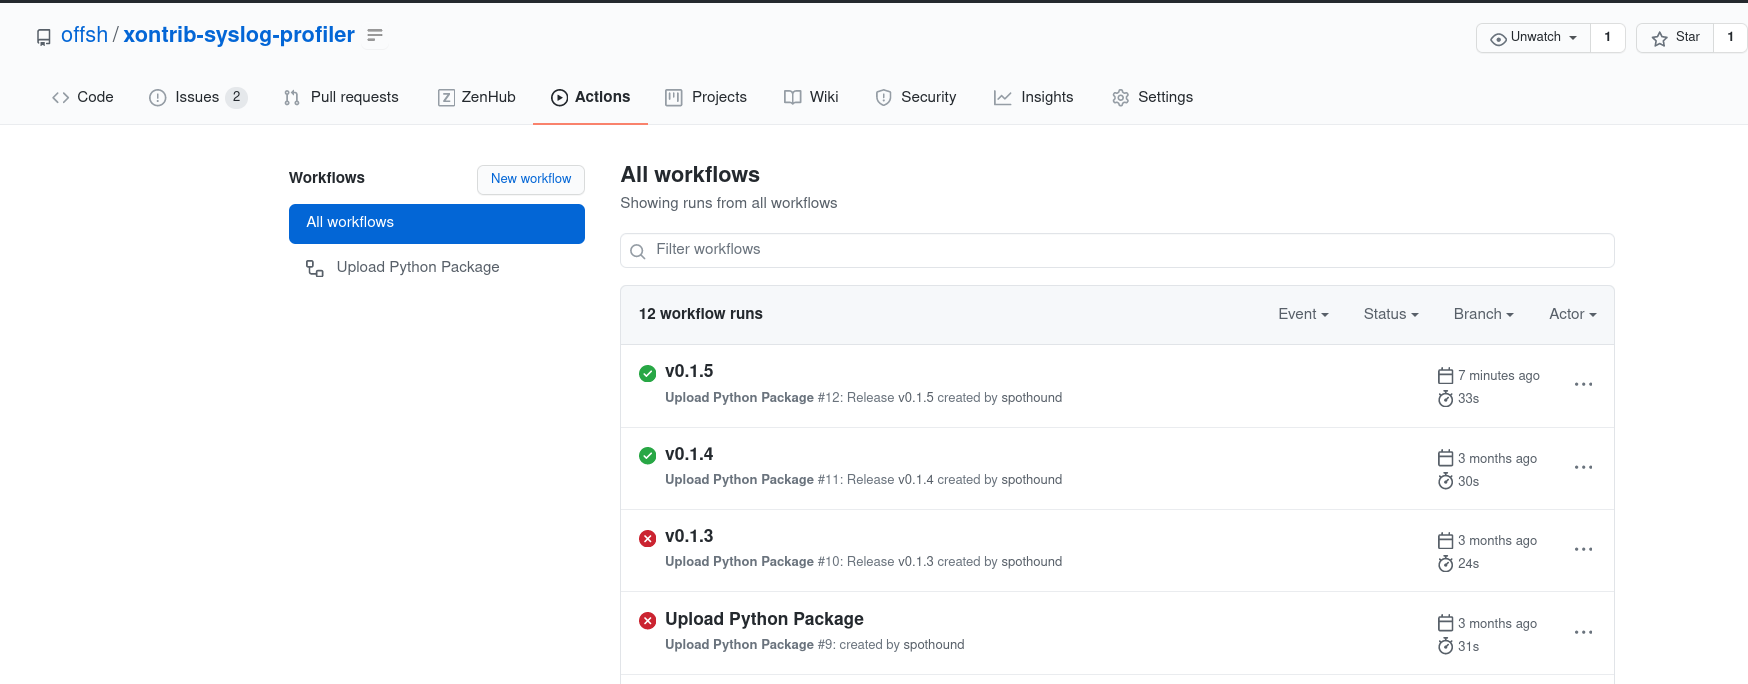
\includegraphics[width=\textwidth]{imagenes/githubactions.png}
  \caption{Ejemplo del uso de Github actions para el despliegue del plugin en Pypi. En ella se aprecia cómo, de forma automática, Github lanza una serie de scripts cuando se genera un nuevo `tag' del código y sube el nuevo paquete al repositorio de pip.}
  \label{githubactions}
\end{figure}

Este plugin hace que todos los comandos ejecutados en Xonsh se guarden en un registro (común a todas las terminales). Basta con instalar el plugin y activarlo en el archivo de configuración de Xonsh para empezar a generar los registros en un fichero predeterminado.

Además, el proyecto incluye un archivo especial de configuración con algunas opciones interesantes para darle un aspecto visual diferente al shell original. Entre estas mejoras, se ha añadido un prompt en forma de barra, que asigna un color aleatorio (dentro de un rango, acorde con el fondo) al nombre de usuario, dominio y directorio activo. De esta forma, cuando se pasa de un host a otro utilizando xxh, se puede apreciar fácilmente el cambio de host y/o de usuario (ver Figura \ref{offsh_example}).


\begin{figure}[!hbt]
  \centering
  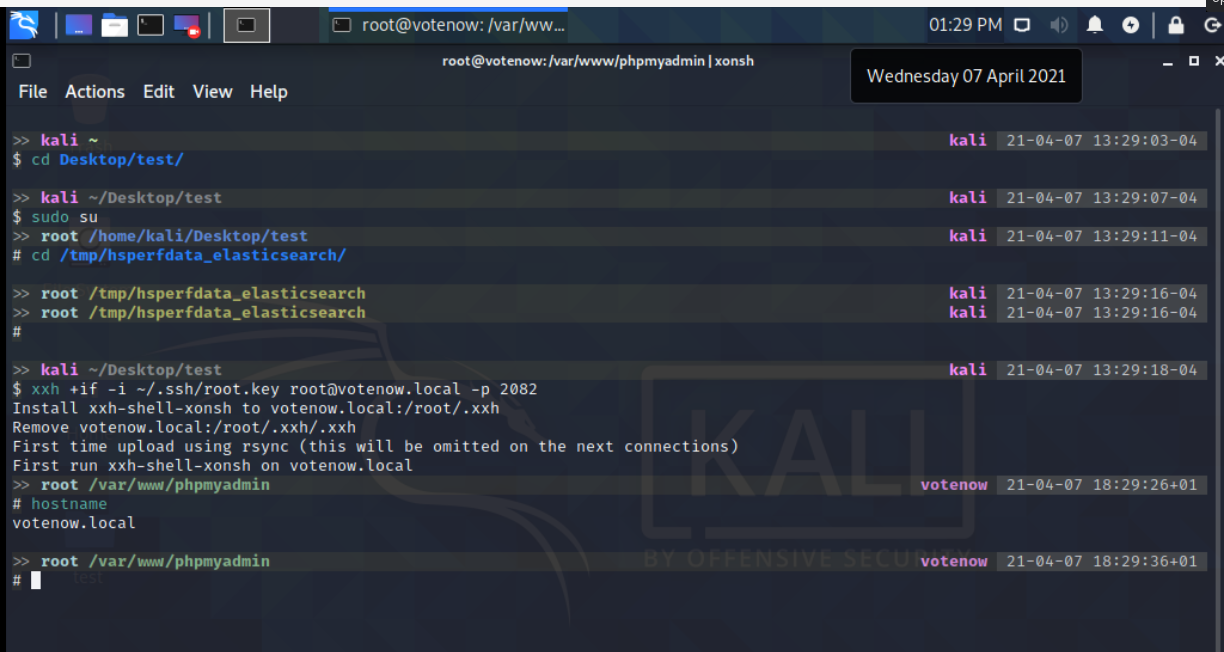
\includegraphics[width=\textwidth]{imagenes/offsh_Example.png}
  \caption{Visualización del uso de offsh con un cambio de host usando xxh. En la imagen se aprecia como el prompt (en barra) muestra el usuario activo, el hostname, directorio actual y el momento de ejecución de cada comando. Esta información (excepto el tiempo) tiene un color determinado por un hash del nombre (de usuario, hostname o path) de forma que el color cambia cuando alguno de estos aspectos cambia también.}
  \label{offsh_example}
\end{figure}


\subsection{Otros usos para el framework}

El framework desarrollado permite montar imágenes modificadas de Xonsh con las características y plugins que se quieran. Como además el plugin que registra los logs que se ha diseñado utiliza el formato syslog, esta funcionalidad podría integrarse con \textbf{cualquier otro software además de Wazuh}. Y los shells creados podrán usarse para distintas funcionalidades.

\begin{figure}[!hbt]
  \centering
  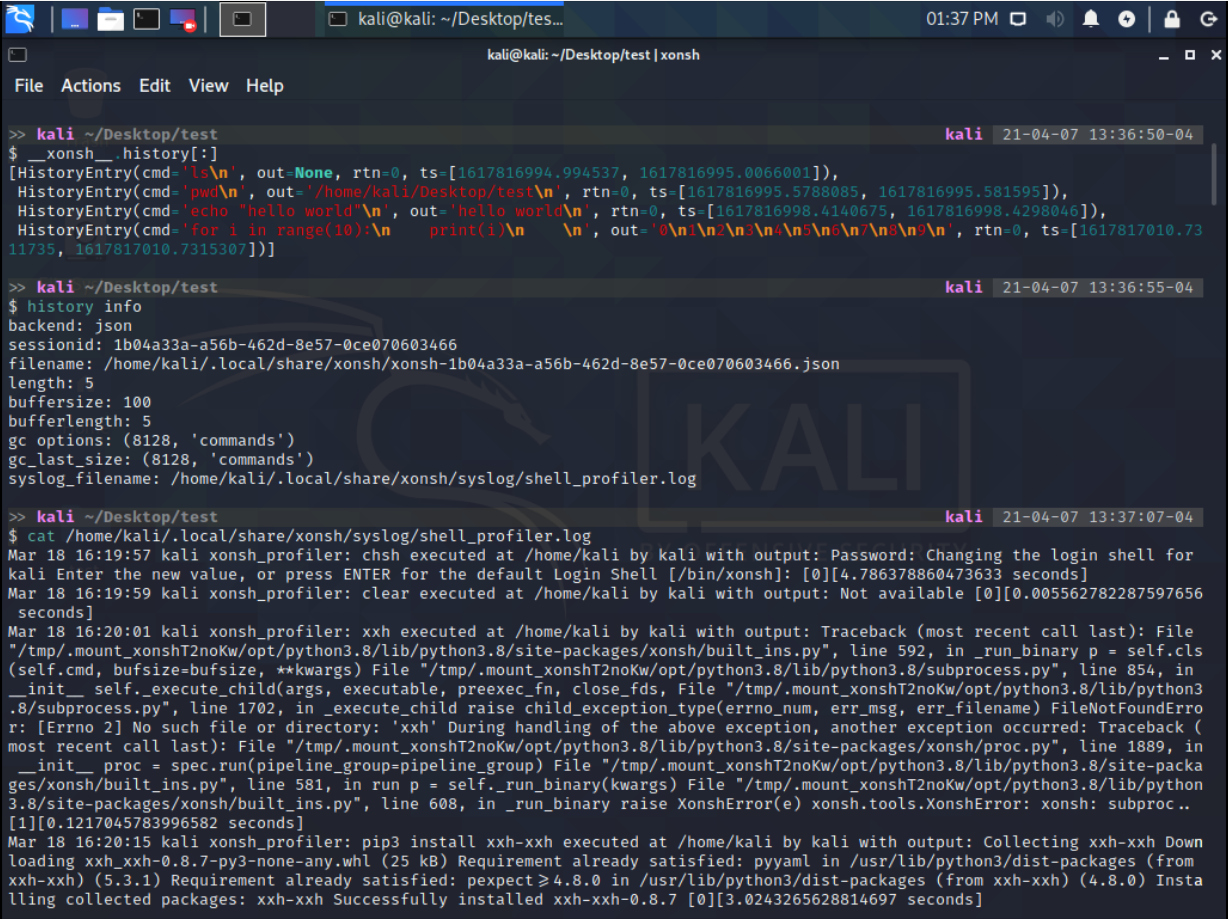
\includegraphics[width=\textwidth]{imagenes/syslog_plugin.png}
  \caption{Ejemplo del fichero generado por el plugin, así como de la forma que tiene Xonsh de almacenar la información (como un objeto Python). En el primer comando ejecutado se ve un mapa con los comandos y sus metadatos, a continuación se usa `history info' para obtener información del backend del historial de Xonsh y se hace un cat del archivo de syslog generado, que contiene la información con el formato que genera el plugin de syslog.}
  \label{syslog_plugin}
\end{figure}

En el apendice \ref{ISE} se expone un ejemplo del uso del mismo, con una propuesta de texto que podría ser incluido en las prácticas de la asignatura de Ingeniería de Servidores (ISE) del Grado en Ingeniería Informática de la Universidad de Granada, con o sin modificaciones. Así como un ejemplo en la Figura \ref{syslog_plugin} de los logs generados.





\subsection{Envío de los logs a Wazuh}

Sobre el envío de los registros a Wazuh, ya se ha discutido en el capítulo anterior (sección \ref{sec:wazuh_kali}) cuales serían las alternativas posibles. Básicamente se trata de enviar el fichero generado por Xonsh al manager, bien usando el agente de Wazuh o un cliente de syslog. Para el caso de uso práctico del capítulo final, por simplicidad, utilizaremos la otra opción propuesta: instalar \textbf{directamente el Wazuh Manager} en el entorno con Xonsh y configurarlo para que lea directamente el archivo con los registros.

La configuración necesaria está brevemente explicada en el repositorio de Github y es la que aparece en el Listado \ref{wazuh_conf}.

\begin{lstlisting}[language=bash,caption={Configuración necesaria para que Wazuh analice los logs generados por Xonsh}, label=wazuh_conf]
<localfile>
  <location>/home/*/.local/share/Xonsh/syslog/shell_profiler.log</location>
  <log_format>syslog</log_format>
</localfile>
\end{lstlisting}



\section{Análisis de los registros y generación de alertas}

Para que Wazuh pueda analizar los registros generados e indexarlos necesitamos algunas reglas y decodificadores adicionales en el conjunto de reglas ($ruleset$) de Wazuh.

Se utilizará un único decoder base (puesto que hemos configurado el plugin de Xonsh para escribir en el registro todos los registros con el mismo formato) que extraiga la información relevante de los comandos  una regla sencilla para generar alertas con la ejecución de comandos. A continuación, se desarrollarían alertas más concretas para determinados comandos o salidas de los mismos e incluso se podrían hacer decodificadores ({\it decoders}) especiales para \textbf{extraer información adicional de la ejecución del comando} como por ejemplo opciones utilizadas o algún elemento interesante de la salida del mismo.

Un detalle importante a tener en cuenta es que el sistema de análisis de registros de Wazuh funciona con una lógica estructurada en árboles de decisión para generar las alertas. Una vez un registro es decodificado por un decoder, se comprueba si concuerda con alguna de las reglas del primer nivel y, si lo hace, entonces se evalúan reglas hijas de la regla que ha coincidido con el registro. Se repite el proceso hasta que no hay más reglas hijas que concuerden con el log y entonces se \textbf{genera una única alerta} a partir de esta última regla. Ver Figura \ref{wazuhtree} para un ejemplo ilustrado.

Teniendo esto en cuenta, podemos crear distintas alertas cada vez más específicas y con distintos grupos y niveles según lo importante que pueda ser la ejecución de ese comando y el tipo de acción que se lleva a cabo. Por ejemplo, algunos grupos en los que agrupar alertas podrían ser:

\begin{itemize}
    \item reconocimiento
    \item ocultación
    \item vulnerabilidades
    \item escalada de privilegios
\end{itemize}

Y según la importancia de cada evento se le asignaría un nivel u otro a la alerta.


\begin{figure}[!hbt]
  \centering
  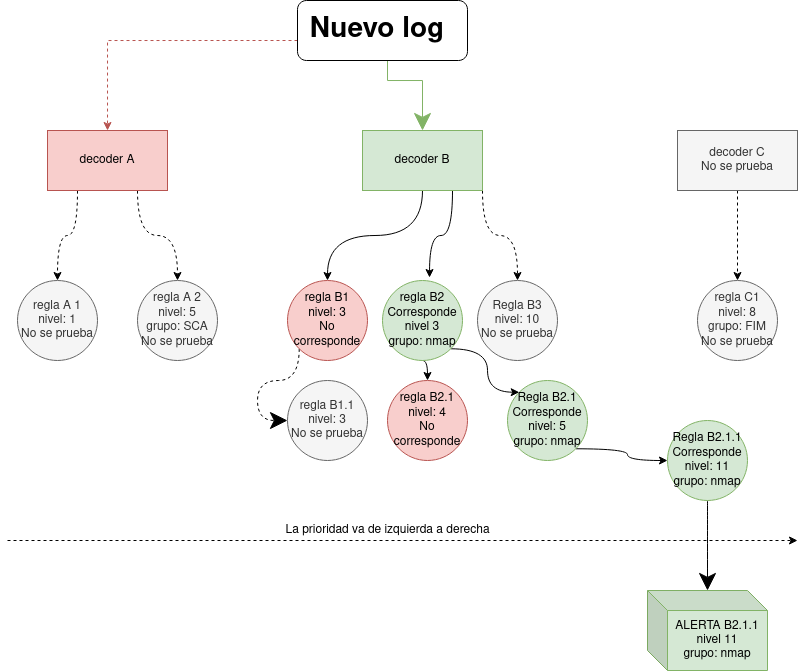
\includegraphics[width=\textwidth]{imagenes/arbol_wazuh.png}
  \caption{Ejemplo gráfico de cómo funciona la lógica de alertas y decoders de Wazuh. Cada decoder tiene una o varias reglas asociadas y estas pueden o no tener hijas. Se van leyendo los decoders hasta que uno coincide con el log de entrada, entonces se van leyendo las reglas en orden hasta que una coincide y esto se repite con las hijas de esta regla hasta que una ya no tiene más hijas (que coincidan con el log), entonces se genera una alerta basada en esa regla.}
  \label{wazuhtree}
\end{figure}




\section{Trabajar con logs de dispositivos externos utilizando XXH}

Ya hemos hablado de XXH, un proyecto complementario a Xonsh que nos permite utilizar una imagen portable de Xonsh (con un \textbf{Python embebido} que nos permite ejecutarlo sin necesidad de tener Python en el sistema) en hosts remotos a los que conectemos por SSH. 


Una primera decisión a tener en cuenta sería \textbf{cómo y cuando obtener los logs de las sesiones externas}, es decir, aunque se use XXH para ejecutar una versión portable de Xonsh que registre la información de los comandos en un fichero remoto (en la máquina accedida), se necesita un mecanismo para enviar dichos logs de nuevo al dispositivo desde el que se abrió la conexión.

La opción más transparente al usuario es modificar XXH para que utilice los mismos credenciales y protocolos que utiliza para \textbf{enviar la imagen portable de Xonsh} y descargue los registros generados en el dispositivo remoto.

Para ello se ha diseñado una versión de XXH\footnote{\url{https://github.com/offsh/xxh}} (a partir de un \gls{fork}) con las modificaciones necesarias para poder ejecutar `plugins' que permitan reutilizar los credenciales de conexión para establecer segundas conexiones de ssh o tcp/rsync, que se usarían para obtener los logs. Además, he creado un plugin\footnote{\url{https://github.com/offsh/xxh-plugin-local-syslog-profiler}} que permite descargar los registros generados en el dispositivo remoto. 



Además, se ha diseñado un pequeño archivo de configuración\footnote{\url{https://github.com/offsh/offsh/blob/main/Xonshrc}} para Xonsh, con algunas modificaciones para mejorar la experiencia de usuario (un prompt visualmente atractivo, colores diferentes según el host en el que estemos trabajando y el nombre de usuario, etc..), plugins de Xonsh que pueden resultar útiles durante las auditorías, alias y demás.

Otra opción que también se ha barajado sería crear un plugin o una funcionalidad para Xxh de `directorios compartidos'. Al igual que hacen algunos software de virtualización (como Virtualbox o Docker), aprovechando la potencia de XXH se podría plantear dicho módulo y utilizarlo para \textbf{sincronizar en tiempo real los resultados de las sesiones remotas}. Esta funcionalidad no se ha implementado como parte del proyecto pero se valora como una posible alternativa de mejora para la opción (más simple) escogida.

De cualquier modo, XXH es una herramienta que se ha incluido de forma nativa (el fork creado a partir de la rama principal de desarrollo) en el framework puesto que consideramos que las funcionalidades que aportan son muy importantes para el desarrollo de distintas consolas de comandos que puedan construirse con las herramientas diseñadas.

Para más información, ver figuras \ref{infographic} y \ref{diagramica}

\begin{figure}[!hbt]
  \centering
  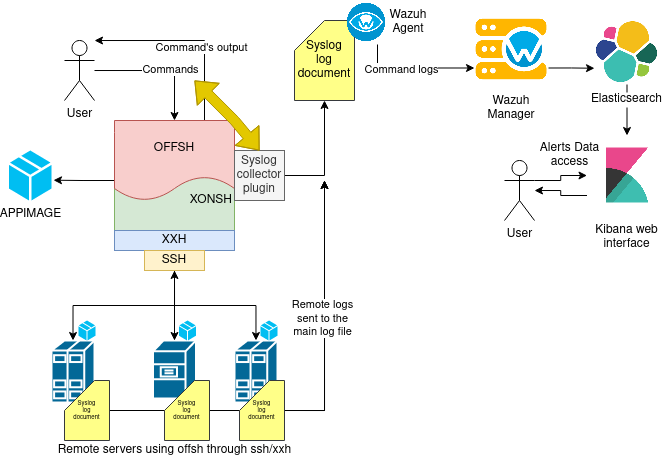
\includegraphics[width=\textwidth]{imagenes/diagramaflujo.png}
  \caption{Diagrama de flujo de datos e información en el que se visualizan las distintas partes del proyecto y cómo interaccionan entre sí. }
  \label{diagramica}
\end{figure}


\begin{figure}[!hbt]
  \centering
  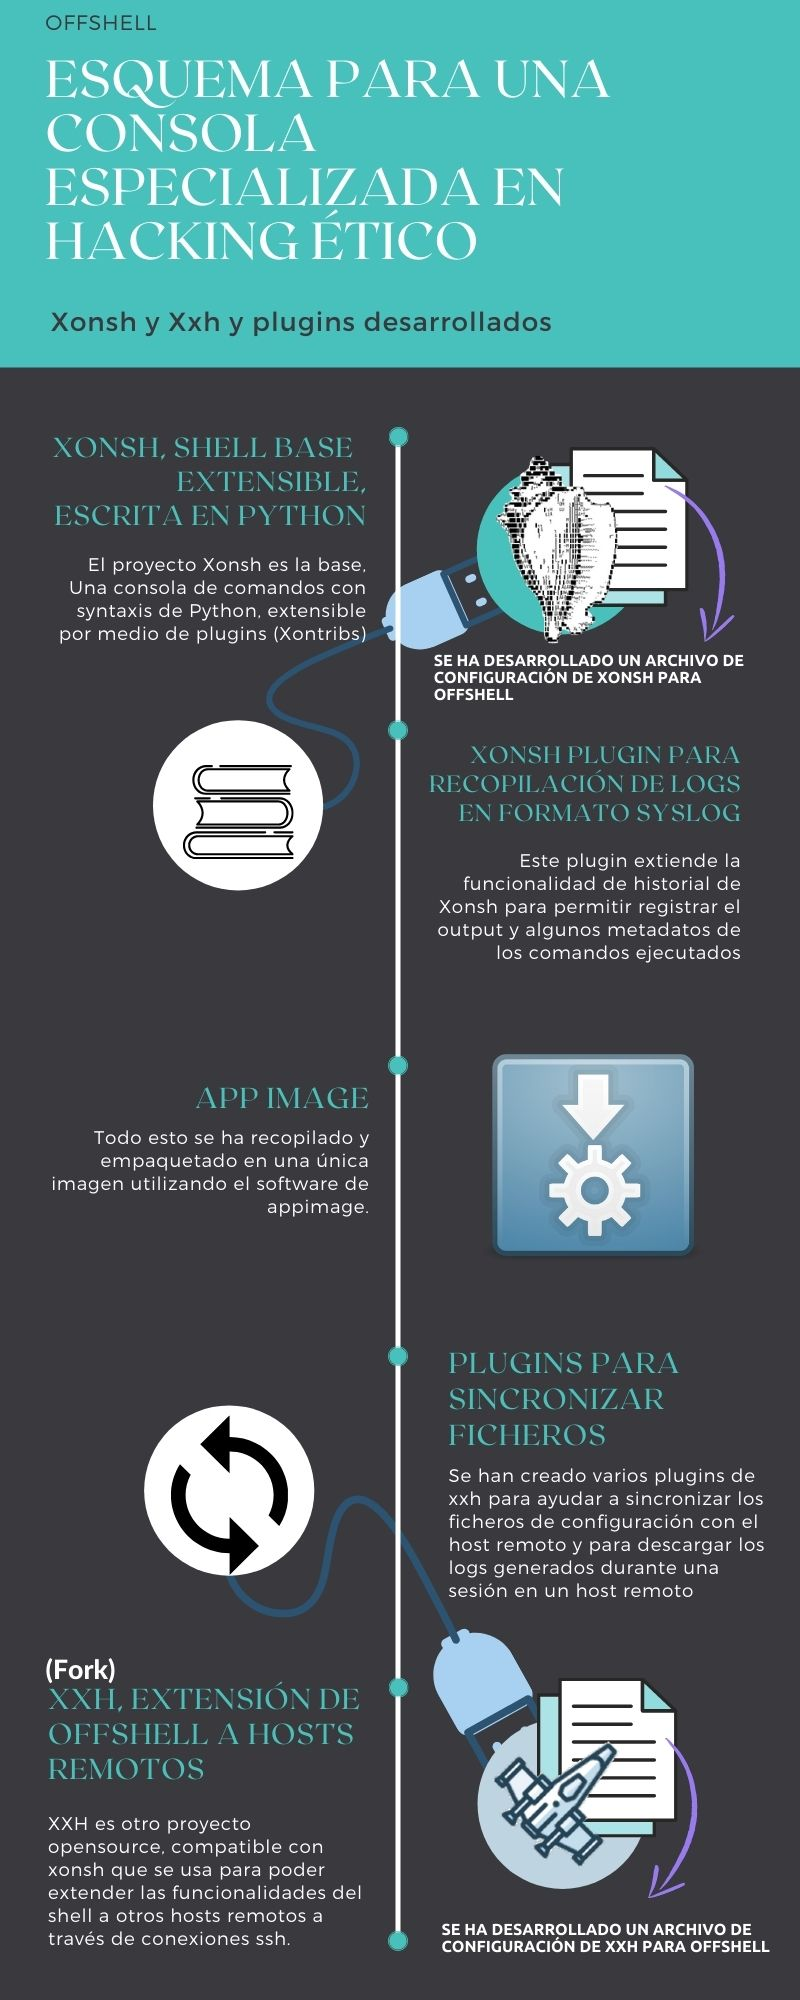
\includegraphics[width=0.5\textwidth]{imagenes/infografico.jpg}
  \caption{Gráfico con información de la estructura y extensiones del proyecto OffSh (Offensive Shell).}
  \label{infographic}
\end{figure}

Xonsh es una herramienta versátil, a la que se pueden añadir fácilmente plugins con nuevas funcionalidades. Es por ello que supone  \textbf{una buena oportunidad para la creación de una consola de comandos especializada en ciberseguridad}. 

Podemos, por tanto, definir una imagen de consola de comandos de offsh como un paquete instalable en cualquier sistrma operativo compatible con Python (que además, incluye una versión embebida de Python para evitar problemas con la versión del sistema operativo dónde se ejecuta), con soporte para usar XXH y archivos de configuración específicos (de Xonsh y XXH), plugins para ambos software y software adicional (por ejemplo, paquetes de python instalados en el python embebido, o binarios incluidos en el paquete con software específico para alguna tarea) que se encapsulan dentro de un paquete del tipo `appimage`.

Algunas de las ideas que se proponen para distinguir este de cualquier otro shell serían:

\begin{itemize}
    \item Un soporte específico para creación de \gls{reverse_shell} que permita crear fácilmente una conexión a través de xxh con un dispositivo en el que se consiga ejecutar código arbitrario, facilitando el acceso a determinadas herramientas dentro del mismo (como nmap u gobuster u otras herramientas útiles para analizar redes internas) y la experiencia de usuario (muy mala en muchas ocasiones por las condiciones visuales y de usabilidad de las shell inversas.
    \item Añadir utilidades de Python relacionadas con la ciberseguridad que se integren con la imagen de Xonsh específica para seguridad, de forma que sean accesibles sin necesidad de instalación. Programas típicos que no pesen mucho, alias, shortcuts, etc..
    \item Aprovechar que Xonsh tiene una base de \textbf{prompt\_toolkit} para añadir prompts dinámicos con información útil sobre los hosts analizados, colores para resaltar información importante, etc..
    \item Añadir scripts en pytest que realicen checks en el servidor en el que se ejecutan o en uno externo y generen alertas en Wazuh si se cumplen determinadas condiciones (automatización de la búsqueda de errores.
    \item Integraciones directas con softwares de ciberseguridad como Wazuh o Elastic SIEM.
\end{itemize}


\section{Simplificación de la instalación: appimage}

Para unificar todo el código desarrollado durante el trabajo tendríamos que conseguir algún tipo de`paquete' instalable que contuviera los siguientes elementos.

\begin{itemize}
    \item Una versión de Xonsh reciente
    \item El archivo de configuración diseñado.
    \item La versión de xxh desarrollada para el proyecto.
    \item El plugin de Xonsh para generar los registros.
    \item El plugin de xxh para descargar los registros externos.
    \item El plugin para analizar el output de determinados comandos.
    \item Otros plugins que puedan ser añadidos en un futuro.
\end{itemize}

Una solución a este problema sería introducir en el archivo de configuración de Xonsh el código necesario para instalar todas estas dependencias si no se encontraran instaladas. Sin embargo, esto tendría el inconveniente de hacer a Xonsh conectarse con hosts remotos para descargar código en la primera ejecución, y esto sería un aspecto negativo cuando se ejecuta Xonsh en una máquina a la que se ha accedido como parte de una auditoría (puesto que estas conexiones podrían ser detectadas).

Sin embargo, siguiendo la documentación de XXH se puede descubrir un elemento interesante: las \textbf{appimages}. Un tipo de empaquetación de software \textbf{portable y multiplataforma} que se puede utilizar sin necesidad de instalarlo ni de permisos de administrador en \textbf{cualquier sistema operativo}.

Xxh hace uso de estas \textit{appimages} para enviar un Xonsh portable y con un \textbf{Python embebido} que hace que podamos \textbf{ejecutar un shell Xonsh en cualquier dispositivo} sin necesidad de tener permisos de administrador o que Python esté instalado o actualizado en el host.

Del mismo modo, Xonsh ofrece un método de `instalación' basado en estas appimages y ofrece \textbf{medios para generar appimages personalizadas de Xonsh}-

Por tanto, la solución obvia parece ser \textbf{crear una appimage} de Xonsh con los elementos ya descritos, de forma que baste con descargarla y ejecutarla. Y que sea esta appimage la que se envía a los dispositivos remotos cuando se establece una conexión utilizando xxh.

Esto refuerza la idea mencionada en el punto anterior de \textbf{la oportunidad de crear un shell específico para penetración de sistemas} que sea portable y fácil de utilizar, y que además facilita la ejecución de código Python, que es un lenguaje muy utilizado en ciberseguridad y pentesting.

La imagen desarrollada, así como las instrucciones para utilizarlas se encuentran en el repositorio: \url{https://github.com/offsh/offsh}. 

\begin{figure}[!hbt]
  \centering
  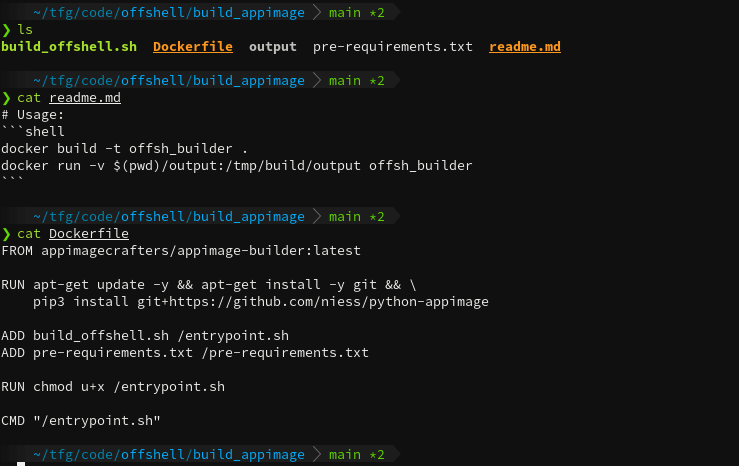
\includegraphics[width=\textwidth]{imagenes/build_appimage.png}
  \caption{Ejemplo de las herramientas y scripts disponibles en el repositorio para generar una nueva appimage de offsh usando Docker.}
  \label{appimage_build}
\end{figure}

La generación de nuevas versiones de la appimage se hace utilizando Docker (para simplificar la obtención de dependencias), tal y como se aprecia en la figura \ref{appimage_build}. Ver también figuras \ref{instructions} (instrucciones de instalación) y \ref{examplexonsh} (ejemplo de visualización de la consola de comandos).

\begin{figure}[!hbt]
  \centering
  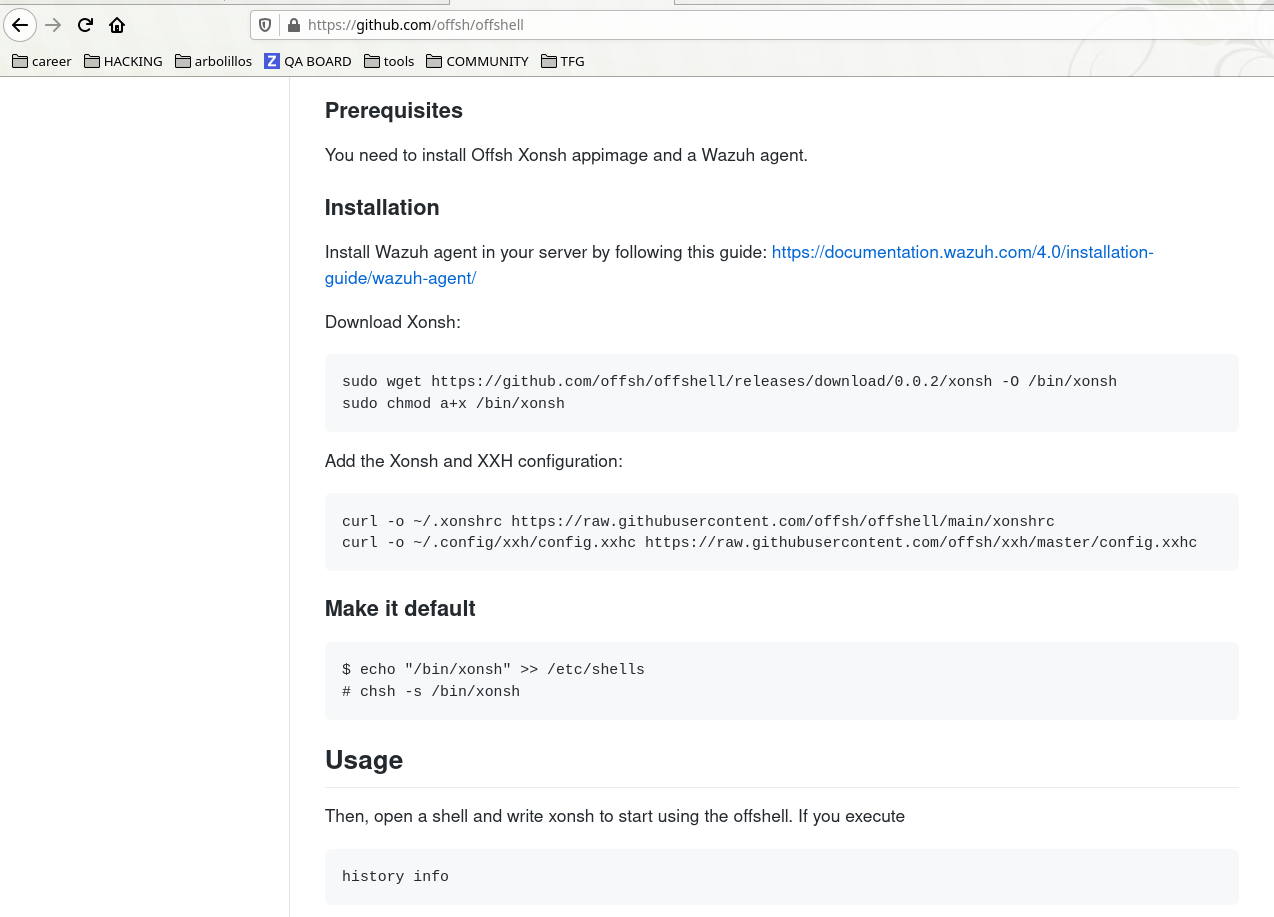
\includegraphics[width=\textwidth]{imagenes/offsh_instructions.png}
  \caption{Instrucciones de instalación y uso de la herramienta, disponibles en github}
  \label{instructions}
\end{figure}

\begin{figure}[!hbt]
  \centering
  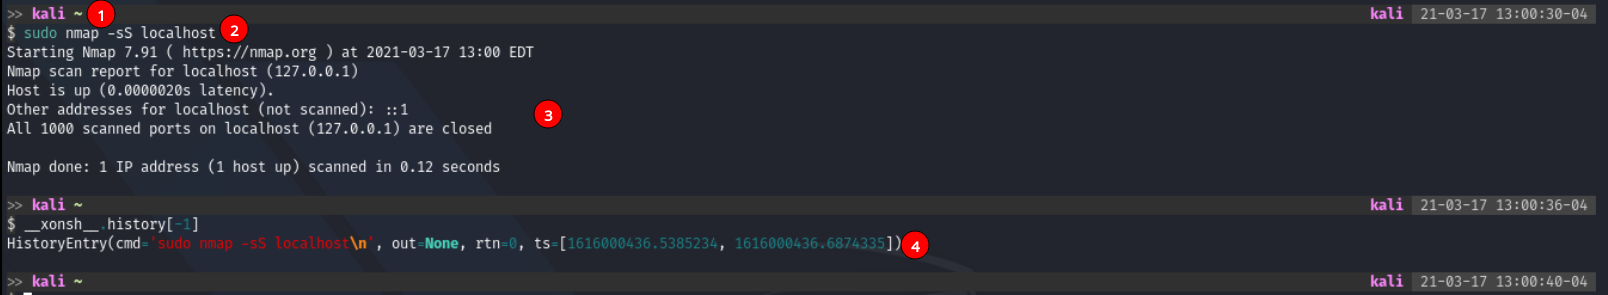
\includegraphics[width=\textwidth]{imagenes/offsh.png}
  \caption{Ejemplo del uso de offsh y la estructura de datos utilizada para almacenar la información de los comandos ejecutados. Se han introducido algunas mejoras visuales al promt de Xonsh por defecto (para diferenciarlo de otras sesiones normales de Xonsh y de otras consolas), como el prompt en barra y los colores según el usuario y el directorio (1). Se aprecia como el comando ejecutado (2) y su output (3) son almacenados en una base de datos que es accesible a través del propio shell (4)}
  \label{examplexonsh}
\end{figure}


\section{Propuesta de aplicación de Offsh para la docencia universitaria}

Para ahondar en la idea de que el proyecto desarrollado puede servir en distintos ámbitos además de en ciberseguridad (y que no se ha creado exclusivamente para ser usado como complemento de Wazuh), se ha decidido realizar una propuesta de aplicación real del mismo para docencia universitaria con ayuda del director de este trabajo, Alberto Guillén, profesor del Departamento de Arquitectura y Tecnología de Computadores que en el momento de la realización del trabajo es responsable de la asignatura de Ingeniería de Servidores.

Para ello, se han analizado los guiones de prácticas actuales de la asignatura y se ha valorado la posibilidad de añadirles el uso de una imagen de xonsh creada con el framework diseñado para el trabajo de forma que los alumnos puedan entender mejor algunos aspectos como:

\begin{itemize}
    \item Qué es un shell y qué diferencia a unos de otros
    \item Ideas básicas sobre archivos de configuración (de un shell, VIM, u otros softwares con archivos similares)
    \item Qué es una conexión ssh, qué implica y cómo puede llevarse a cabo por medio de programas más complejos como xxh
    \item Qué es una consola de comandos, TTY, 
\end{itemize}

\subsection{Propuesta de integración en las prácticas de la asignatura}

En la segunda práctica de la asignatura se trabaja el uso de SSH, la propuesta entonces es la siguiente: añadir una descripción básica de Xonsh y de offsh y xxh así como instrucciones para instalarlo y usarlo dentro de un sistema

\subsection{Desarrollo de competencias}

Con esta propuesta se pretende ayudar a que los alumnos adquieran las siguientes competencias:

\begin{itemize}
    \item Competencias específicas de la asignatura
    \begin{itemize}
        \item \textbf{R1. Capacidad para diseñar, desarrollar, seleccionar y evaluar aplicaciones y sistemas informáticos, asegurando su fiabilidad, seguridad y calidad, conforme a principios éticos y a la legislación y normativa vigente.}, ya que conocerán distintos tipos de shell y podrán elegirlos según sus necesidades y saber cómo configurarlos.
        \item \textbf{R5. Conocimiento, administración y mantenimiento de sistemas, servicios y aplicaciones informáticas.}, ya que los shell y las conexiones ssh son aspectos fundamentales dentro de la administración de sistemas.
    \item Competencias Transversales
    \begin{itemize}
        \item \textbf{ T2. Capacidad de organización y planificación así como capacidad de gestión de la
Información.}, ya que trabajan con mecanismos para registrar la información (Datos y metadatos) generada durante una sesión de ejecución de comandos en una shell.
    \end{itemize}
    \end{itemize}
\end{itemize}

Desde el punto de vista del profesorado, se podrían usar los logs generados por los alumnos para evaluar el cumplimiento de estas y otras competencias, por ejemplo, se podría pasar una batería de tests sobre el fichero de logs generado por cada alumnos para comprobar que, efectivamente, se han cumplido ciertos requisitos para superar las prácticas.
